% This is based on the LLNCS.DEM the demonstration file of % the LaTeX macro
% package from Springer-Verlag % for Lecture Notes in Computer Science, version
% 2.4 for LaTeX2e as of 16. April 2010
%
% See http://www.springer.com/computer/lncs/lncs+authors?SGWID=0-40209-0-0-0
% for the full guidelines.
\documentclass{llncs}
\usepackage{graphicx}
\graphicspath{ {./assets/} }

\usepackage{enumitem}
\setlist[enumerate]{itemsep=2mm}

\usepackage{dirtytalk}
\usepackage{minted}
\usepackage{amsmath}
\usepackage{pdflscape}
\usepackage[pass]{geometry}

%
% Tables
% --------
\usepackage[table]{xcolor}
\usepackage{hhline}
\usepackage{booktabs} % much better tables
\usepackage{multirow} % allows to fuse rows
\usepackage{array}    % manipulate array
\usepackage{tabularx} % better tables

% Define new tabularx column types:
%  - R: streteched right aligned
%  - C: stretched centered
%  - N: left aligned, specified space
\newcolumntype{R}{>{\raggedleft\arraybackslash}X}
\newcolumntype{C}{>{\centering\arraybackslash}X}
\newcolumntype{N}[1]{>{\raggedleft\arraybackslash}p{#1}}
\newcolumntype{S}{>{\hsize=.5\hsize}C}

% Set row height multiplicator to provide more breathing space
\renewcommand{\arraystretch}{1.5}

\usepackage[backend=biber]{biblatex}
\addbibresource{bibliography.bib}

\pagestyle{plain}
\setcounter{page}{1}
\pagenumbering{arabic}

\usepackage{pgfplots}
\pgfplotsset{width=6cm}
\usepackage{float}
\usepackage[caption = false]{subfig}

\begin{document}

\title{Multi-client Partially Non-Interactive and Instantaneous One-way Payment Channel for Ethereum}
\author{Thomas Shababi\inst{1} \and Jo\"el Gugger\inst{1} \and Daniel Lebrecht\inst{1}}

\authorrunning{Thomas~S.~Shababi et al.}
\tocauthor{Thomas~S.~Shababi, Joel Gugger, and Daniel Lebrecht}
\subtitle{{\normalsize\today{\small\ -- DRAFT}}}
\institute{TrueLevel SA, Neuch\^atel, Switzerland\\ \email{\{tom, joel, d\}@truelevel.io}}

\maketitle

\begin{abstract} Ethereum is a distributed computing platform and operating system featuring smart contract functionality. Transactions are faster than other blockchain but not instant and each of them cost some ``gas''. This gas is used to quantify the amount of fee to pay for computation. \keywords{Crypto-currencies, Ethereum, Payment channels}
\end{abstract}

\section{Introduction} 

\subsubsection{Requirements Language}
The key words ``MUST", ``MUST NOT", ``REQUIRED", ``SHALL", ``SHALL NOT",
``SHOULD", ``SHOULD NOT", ``RECOMMENDED", ``MAY", and ``OPTIONAL" in this
document are to be interpreted as described in RFC 2119 \cite{Bradner1997}.

\section{Multi-clients payment channels} Partially non-interactive multi-clients payment channels are composed of clients $c \in \mathcal{C}$ and one provider $\mathcal{P}$. $\mathcal{C}$ is the set of all clients registred in the multi-clients payment channel. Clients can send money to the provider through the channel $c \rightarrow \mathcal{P}$ but cannot recieve through the channel $\mathcal{P} \not\rightarrow c$.

A payment channel is by definition a structure composed of two layers of states. The first layer of states is registered to the blockchain, i.e. ``on-chain'' or contract states $\mu \in M$, and the second layer of states is kept ``off-chain'' between the participants, i.e. channel states $\sigma \in \Sigma$.

It is possible to transition from a state $\sigma$ to another state $\sigma'$. We denote state transition with $\rightarrow$, i.e. $\sigma \rightarrow \sigma'$.  Modifiers $\omega \in \Omega$ are used to create transition on channel states $\sigma \in \Sigma$. A transition in $\Sigma$ depends on modifiers and contract states. We denote a transition from $\sigma, \sigma' \in \Sigma$ that depends on $\mu \in M$ and $\omega \in \Omega$ as
$$\sigma \xrightarrow{\mu+\omega} \sigma'$$

Contract state transitions are triggered by external events $e \in \mathcal{E}$ or messages $m \in \mathcal{M}$. Transitions between two states $\mu, \mu' \in M$ are denoted $\mu \rightarrow \mu '$. If the transition is due to an external event $e$ we write $\mu \xrightarrow{e} \mu '$. If the transition is due to a message $m$ we write $\mu \xrightarrow{m} \mu '$. Generic transitions are noted as $\mu \rightarrow \mu '$.

A message $m$ can be ``applied'' to a state $\mu$, we denote this operation with $m(\mu)$, i.e. $\mu \xrightarrow{m} \mu'$. Messages are created based on a channel states. Each channel state $\sigma \in \Sigma$ can derive its corresponding message $m \in \mathcal{M}$
$$\forall \sigma \in \Sigma,\ \exists m\ |\ m \in \mathcal{M}$$

In reality it is not necessary to derive all messages. External events (top ups) afect the channel state but no messages are created because the previous generated message is still valid and usable to trigger a valid state transition in $M$.

\subsection{Contract state variables} We define variables to acces the the contract state $\mu \in M$ for a client $c \in \mathcal{C}$.

\subsubsection{Current on-chain index, $I(c)$} For each client the current index $i$ must be retreivable, $\forall c \in \mathcal{C}, \quad \exists I(c) \in \mu >= 0$. The index for a client must start from $0$.

\subsubsection{Current on-chain balance, $B_\mu(c)$} For each client the current balance amount must be retreivable, $\forall c \in \mathcal{C}, \quad \exists B_\mu(c) \in \mu >= 0$.

\subsubsection{Refund parameters, $R(c)$} For each client the current refund parameters must be retreivable, $\forall c \in \mathcal{C}, \quad \exists R(c) \in \mu$ such that $R(c)$ is the provider owned amount at the moment of the requested refund. The remaing money must go to the client.

\subsection{Contract states} Each client $c \in \mathcal{C}$ in the contract is defined by an on-chain state $\mu \in M$. States $\mu \in M$ are a tuple
$$(I(c), B_\mu(c), R(c))$$

\subsection{Channel state variables} We define variables to represent: (i) the lifetime of a single channel in the multi-clients channel architecture, (ii) the total amount deposited for a client over the lifetime, (iii) the total amount own by the provider over the lifetime, and (iv) the minimal and full available amount for the client.

\subsubsection{Channel lifetime, $L(c \rightarrow \mathcal{P})$} It exists one lifetime and only one per element in $\mathcal{C} \times \mathcal{P}$ and begins when the first deposit is made, i.e. one lifetime per client $c \in \mathcal{C}$.

\subsubsection{Total deposit, $D(c)$} Total deposit of a client $c$ represents the total amount recieved from the begining of the lifetime. Each top up increases the total deposit.

\subsubsection{Total sent, $\sum c \rightarrow \mathcal{P}$} Total amount sent to the provider by a client $c$ represents the sum of all transaction since the begining of the lifetime. Each transaction increases the total sent.

\subsubsection{Minimal available amount, $A_m(c)$} Minimal amount available for a client $c$ is computed with the latest channel state $\sigma$. Without quering the contract state $\mu$ it is impossible to know if a bigger amount is now available. The minimal available amount is computed with
$$A_m(c) = D(c) - \textstyle \sum c \rightarrow \mathcal{P}$$

\subsubsection{Client available amount, $A(c)$} The full amount available into a single channel for a client $c \in \mathcal{C}$ is computed with
$$A(c) = D(c) - \textstyle \sum c \rightarrow \mathcal{P} + (B_\mu(c) - B_\sigma(c)), \quad B_\mu(c) \geq A(c)$$

It is worth noting that $B_\mu(c) - B_\sigma(c)$ is added to the difference of total deposit and total sent in case of on-chain changements, like top up.

\subsection{Channel states} Each client $c \in \mathcal{C}$ is defined by their channel state $\sigma \in \Sigma$. States $\sigma \in \Sigma$ are composed of: (i) a validity index, (ii) the latest observed on-chain balance
of the client, (iii) the total deposit of the client, and (iv) the total owned by the provider. We denote a state $\sigma \in \Sigma$ as
$$(i, B_\sigma(c), D(c), \textstyle \sum c \rightarrow \mathcal{P})$$

\subsection{Messages} Messages $m \in \mathcal{M}$ are exchanged between clients $\mathcal{C}$ and provider $\mathcal{P}$. A message is related to one and only one element in $\mathcal{C} \times \mathcal{P}$.

\subsubsection{Minimal message} A minimal message $m \in \mathcal{M}$ between a client $c$ and the provider $\mathcal{P}$ is composed of four components: (i) a validity index, (ii) the lastest observed balance, (iii) the total of deposit, and (iv) the total owned by the provider. We denote a message $m \in \mathcal{M}$ as
$$(i, B_\sigma(c), D(c), \textstyle \sum c \rightarrow \mathcal{P})$$

\subsubsection{Message derivation} Messages are derived from channel states $\Sigma$ as
\begin{equation*}
\begin{split}
    \sigma &\implies m \\
    (i, B_\sigma(c), D(c), \textstyle \sum c \rightarrow \mathcal{P}) &\implies (i+1, B_\sigma(c), D(c), \textstyle \sum c \rightarrow \mathcal{P}) \\
\end{split}
\end{equation*}

\subsection{Modifiers} Modifiers $\omega \in \Omega$ are input parameters that modify channel states $\sigma$. They encapsulate the channel capabilities. In this multi-clients payment channel the capability is sending money through the channel from clients to provider, i.e. $c \rightarrow \mathcal{P}$.

\subsubsection{Payment, $\omega(a)$} This modifier is used to increase the balance $O(\mathcal{P})$ of the provider of $a$ amount from a client $c$.

\section{State transitions}

\subsection{Contract state, $\mu \rightarrow \mu'$} Contract states $\mu \in M$ can transition $\mu \rightarrow \mu'$ because of a message $m \in \mathcal{M}$ or external events.

\begin{figure}[h]
\subfloat[Valid transitions in $M$]{
    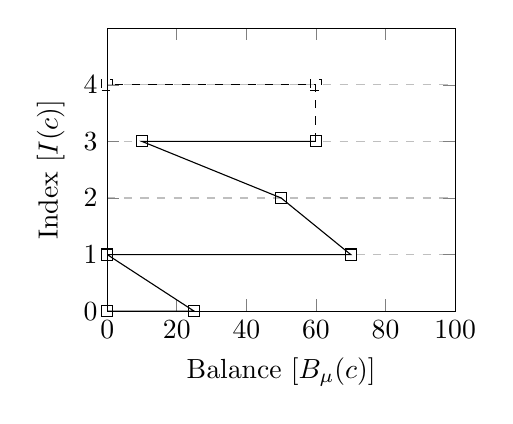
\begin{tikzpicture}
    \begin{axis}[
        xlabel={Balance [$B_\mu(c)$]},
        ylabel={Index [$I(c)$]},
        xmin=0, xmax=100,
        ymin=0, ymax=5,
        xtick={0,20,40,60,80,100},
        ytick={0,1,2,3,4},
        ymajorgrids=true,
        grid style=dashed,
    ]
     
    \addplot[
        color=black,
        mark=square,
        ]
        coordinates {
            (0,0)(25,0)(0,1)(70,1)(50,2)(10,3)(60,3)
        };

    \addplot[
        color=black,
        mark=square,
        dashed,
        ]
        coordinates {
            (60,3)(60,4)(0,4)
        };
     
    \end{axis}
    \end{tikzpicture}}
\subfloat[$(I(c), B_\mu(c)) \rightarrow (I(c)+1, B_\mu(c)\uparrow)$]{
    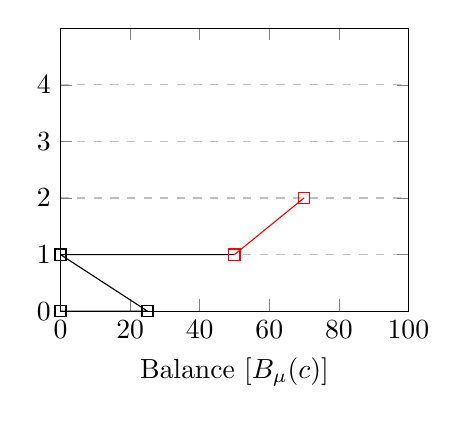
\begin{tikzpicture}
    \begin{axis}[
        xlabel={Balance [$B_\mu(c)$]},
        xmin=0, xmax=100,
        ymin=0, ymax=5,
        xtick={0,20,40,60,80,100},
        ytick={0,1,2,3,4},
        ymajorgrids=true,
        grid style=dashed,
    ]
     
    \addplot[
        color=black,
        mark=square,
        ]
        coordinates {
            (0,0)(25,0)(0,1)(50,1)
        };
     
    \addplot[
        color=red,
        mark=square,
        ]
        coordinates {
            (50,1)(70,2)
        };
     
    \end{axis}
    \end{tikzpicture}}\\
\subfloat[$(I(c), B_\mu(c)) \rightarrow (I(c)\downarrow, \_)$]{
    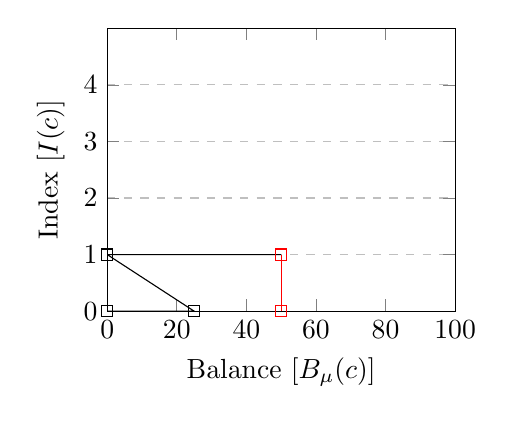
\begin{tikzpicture}
    \begin{axis}[
        xlabel={Balance [$B_\mu(c)$]},
        ylabel={Index [$I(c)$]},
        xmin=0, xmax=100,
        ymin=0, ymax=5,
        xtick={0,20,40,60,80,100},
        ytick={0,1,2,3,4},
        ymajorgrids=true,
        grid style=dashed,
    ]
     
    \addplot[
        color=black,
        mark=square,
        ]
        coordinates {
            (0,0)(25,0)(0,1)(50,1)
        };
     
    \addplot[
        color=red,
        mark=square,
        ]
        coordinates {
            (50,1)(50,0)
        };
     
    \end{axis}
    \end{tikzpicture}}
\subfloat[$(I(c), B_\mu(c)) \rightarrow (I(c), B_\mu(c)\downarrow)$]{
    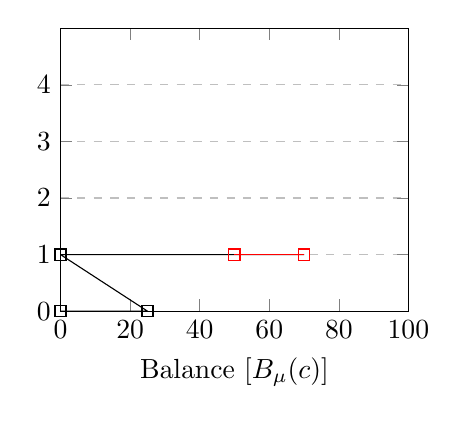
\begin{tikzpicture}
    \begin{axis}[
        xlabel={Balance [$B_\mu(c)$]},
        xmin=0, xmax=100,
        ymin=0, ymax=5,
        xtick={0,20,40,60,80,100},
        ytick={0,1,2,3,4},
        ymajorgrids=true,
        grid style=dashed,
    ]
     
    \addplot[
        color=black,
        mark=square,
        ]
        coordinates {
            (0,0)(25,0)(0,1)(70,1)
        };
     
    \addplot[
        color=red,
        mark=square,
        ]
        coordinates {
            (70,1)(50,1)
        };
     
    \end{axis}
    \end{tikzpicture}}
\caption{State transitions in $M$, transitions in red are not allowed. Dashed transition are during refund process. The first step is the refund request, the second can be either claim, resolve, or dispute.}
\label{fig:contractStateTransitions}
\end{figure}

\subsubsection{Settlement} $(I(c), B_\mu(c), R(c)) \xrightarrow{m} (I(c)+1, B_\mu(c)\downarrow, R(c))$ where
$$m = (i, B_\sigma(c), D(c), \textstyle\sum c \rightarrow \mathcal{P})\ |\ i = I(c)+1$$

It is worth noting that with this rule it is not possible to settle a zero amount because the balance amount $B_\mu(c)$ must go down!
\begin{equation*}
\begin{split}
    O(\mathcal{P}) &= B_\mu(c) - A(c) \\
    &= B_\mu(c) - (D(c) - \textstyle \sum c \rightarrow \mathcal{P} + (B_\mu(c) - B_\sigma(c))) \\
\end{split}
\end{equation*}

$O(\mathcal{P})$ is the amount owned by the provider at the settlement time. The provider can settle the amount in the balance minus the remaining funds of the client $c$.
\begin{equation*}
\begin{split}
    B_\mu(c)\downarrow \ &= B_\mu(c) - O(\mathcal{P}) \\
    &= B_\mu(c) -(B_\mu(c) - (D(c) - \textstyle \sum c \rightarrow \mathcal{P} + (B_\mu(c) - B_\sigma(c)))) \\
\end{split}
\end{equation*}

The new client balance is the current contract balance minus the the amount due to the provider.

\subsubsection{Refund} $(I(c), B_\mu(c),R(c)) \xrightarrow{m} (I(c)+1, B_\mu(c), R(c)')$ where
$$m = (i, B_\sigma(c), D(c), \textstyle\sum c \rightarrow \mathcal{P})\ |\ i = I(c)+1$$

It is a full refund if the client available funds in the channel for the client are equal to the current contract balance and a partial refund if the available funds of the client are smaller than the balance
\begin{equation*}
\begin{split}
    R(c)' &=
  \begin{cases}
      B_\mu(c) - A(c) & \quad \text{if } B_\mu(c) > A(c) \\
      0 & \quad \text{if } B_\mu(c) = A(c) \\
  \end{cases}
\end{split}
\end{equation*}

%\begin{equation*}
%\begin{split}
%    B_\mu(c) &\overset{?}{=} A(c) \\
%    &\overset{?}{=} D(c) - \textstyle \sum c \rightarrow \mathcal{P} + (B_\mu(c) - B_\sigma(c)) \\
%\end{split}
%\end{equation*}
%
%In that case 
%$$R(c)' = (0,d)\ |\ d = \texttt{current\_block\_number} + \texttt{delay}$$
%
%If the client available funds in the channel are smaller than the current contract balance it is a partial refund
%\begin{equation*}
%\begin{split}
%    B(c) &\overset{?}{>} A(c)
%\end{split}
%\end{equation*}
%
%In that case the provider amount is
%\begin{equation*}
%\begin{split}
%    R(c)' &= (O(\mathcal{P}),d) \\
%    d &= \texttt{current\_block\_number} + \texttt{delay} \\
%    O(\mathcal{P}) &= B_\mu(c) - A(c)
%\end{split}
%\end{equation*}

\subsubsection{Dispute} $(I(c), B_\mu(c),R(c)) \xrightarrow{m} (I(c), 0, 0)$ where
$$m = (i, B_\sigma(c), D(c), \textstyle\sum c \rightarrow \mathcal{P})\ |\ i = I(c)$$

If $O(\mathcal{P}) > R(c)$ the provider won the dispute and $O(\mathcal{P})$ is transfer to the provider plus some penalities, the rest is sent to the client.

\subsubsection{Resolve} $(I(c), B_\mu(c),R(c)) \xrightarrow{m} (I(c), 0, 0)$ where
$$m = (i, B_\sigma(c), D(c), \textstyle\sum c \rightarrow \mathcal{P})\ |\ i = I(c)$$

If $O(\mathcal{P}) = R(c)$ the provider accept the refund. $O(\mathcal{P})$ is transfer to the provider and the rest is sent to the client imediately.

\subsubsection{Top up} $(I(c), B_\mu(c),R(c)) \xrightarrow{e} (I(c), B_\mu(c)\uparrow,R(c))$. Top up increases the contract balance for a client $c \in \mathcal{C}$. Validity index $I(c)$ must not be incremented during the top up.

\subsubsection{Invalid settlement} $(I(c), B_\mu(c),R(c)) \rightarrow (I(c), B_\mu(c)\downarrow,R(c))$. This transition is invalid because the balance is decreased without incrementing the validity index $I(c)$. The current set of transactions must be invalidate after the settlement.

\subsubsection{Invalid top up} $(I(c), B_\mu(c),R(c)) \rightarrow (I(c)+1, B_\mu(c)\uparrow,R(c))$. Increasing validity index $I(c)$ while increasing the contract balance invalidates the set of transaction $I(c)$. The current set of transactions must be invalidate only during a settlement.

\subsubsection{Invalid validity index} $(I(c), B_\mu(c),R(c)) \rightarrow (I(c)\downarrow, \_, \_)$. Decreasing the validity index $I(c)$ is always invalid. Validity index must not be decreased.

\begin{table}[t]
  \begin{tabularx}{\textwidth}{| S | S | C | C | C |}
    \cline{2-5}
      \multicolumn{1}{c|}{ } & $\omega$ & $\mu$ & $m$ & $\sigma$ \\ \cline{2-5}
      \multicolumn{1}{c|}{ } & $\omega(a)$ & $(I(c), B_\mu(c),R(c))$ & $(i, B_\sigma(c), D(c), \sum)$ & $(i, B_\sigma(c), D(c), \sum)$ \\
  \hhline{-====}
      init & & $(0,10,0)$ & & $\emptyset$ \\
      transact & $+1$ & & $(1, 10, 10, 1)$& $(0, 10, 10, 1)$ \\
      transact & $+1$ & & $(1, 10, 10, 2)$& $(0, 10, 10, 2)$ \\
      settle & & $(1,8,0)$ & & \\
      transact & $+2$  & & $(2, 8, 10, 4)$ & $(1, 8, 10, 4)$ \\
      transact & $+2$  & & $(2, 8, 10, 6)$ & $(1, 8, 10, 6)$ \\
      top up & & $(1,18,0)$ & & $(1, 18, 20, 6)$ \\
      transact & $+1$ & & $(2, 18, 20, 7)$ & $(1, 18, 20, 7)$ \\
      settle & & $(2,13,0)$ & $(3,13,20,7)$ & $(2,13,20,7)$ \\
      refund & & $(3,13,0)$ & & \\
      claim & & $(3,0,0)$ & & \\
      \cline{1-5}
  \end{tabularx}
  \medskip
  \caption{State transitions during channel lifetime}
\end{table}

\subsection{Channel state, $\sigma \rightarrow \sigma'$} Channel state transitions $\sigma \xrightarrow{\mu + \omega} \sigma'$ for $\sigma, \sigma' \in \Sigma$, i.e. applying a modifier $\omega$ on the current state $\mu$ to result on $\sigma'$. The contract state $\mu$ must be query on-chain. The base channel state is
\begin{equation*}
\begin{split}
  \sigma &=
  \begin{cases}
    \emptyset & \quad \text{if no previous state exists} \\
    (i, B_\sigma(c), D(c), \textstyle \sum c \rightarrow \mathcal{P}) & \quad \text{otherwise}
  \end{cases}
\end{split}
\end{equation*}

\subsubsection{Payment, $\mu(I(c), B_\mu(c), R(c))+\omega(a)$} Payments trigger transition in channel states from a base state $\sigma$ to a destination state $\sigma'$ noted $\sigma \xrightarrow{\mu + \omega(a)} \sigma'$.
The destination state is computed as
\begin{equation*}
\begin{split}
  \sigma' &=
  \begin{cases}
      (I(c), B_\mu(c), B_\mu(c), a) & \quad \text{if } \sigma = \emptyset \\
      (I(c), B_\mu(c), D(c), \textstyle \sum c \rightarrow \mathcal{P}+a) & \quad \text{otherwise}
  \end{cases}
\end{split}
\end{equation*}

\subsubsection{Top up, $\mu(I(c), B_\mu(c) \uparrow, R(c))$} Each top up event modify the contract state $\mu$, then the channel state $\sigma$ must be updated to keep track of the real balance.
\begin{equation*}
\begin{split}
  \sigma' &=
  \begin{cases}
      (I(c), B_\mu(c), B_\mu(c), 0) & \quad \text{if } \sigma = \emptyset \\
      (I(c), B_\mu(c), D(c) + (B_\mu(c) - B_\sigma(c)), \textstyle \sum c \rightarrow \mathcal{P}) & \quad \text{otherwise}
  \end{cases}
\end{split}
\end{equation*}

\begin{table}[t]
  \begin{tabularx}{\textwidth}{| S | S | C | C | C |}
    \cline{2-5}
      \multicolumn{1}{c|}{ } & $\omega$ & $\mu$ & $m$ & $\sigma$ \\ \cline{2-5}
      \multicolumn{1}{c|}{ } & $\omega(a)$ & $(I(c), B_\mu(c),R(c))$ & $(i, B_\sigma(c), D(c), \sum)$ & $(i, B_\sigma(c), D(c), \sum)$ \\
  \hhline{-====}
      init & & $(0,3,0)$ & & $\emptyset$ \\
      top up & & $(0,5,0)$ & & $(0, 5, 5, 0)$ \\
      transact & $+3$ & & $(1, 5, 5, 3)$ & $(0, 5, 5, 3)$ \\
      settle & & $(1,2,0)$ & & \\
      transact & $+1$ & & $(2, 2, 5, 4)$ & $(1, 2, 5, 4)$ \\
      top up & & $(1,4,0)$ & & $(1, 4, 7, 4)$ \\
      settle & & $(2,3,0)$ & & \\
      transact & $+2$ & & $(3, 3, 7, 6)$ & $(2, 3, 7, 6)$ \\
      refund & & $(3,3,2)$ & & \\
      resolve & & $(3,0,0)$ & & $(3,0,7,6)$ \\
      \cline{1-5}
  \end{tabularx}
  \medskip
  \caption{Settlement after top up and refund resolved}
\end{table}

\section{Protocol} The protocol describes interactions between clients and the provider and messages negociation. Protocol introduce a new component in the channel architecture, directives. Directives are the concrete implementation of messages and are distributed between client and provider.

\subsubsection{Client actions} A client can send money through the channel and refund his money after some time if he submited the right message $m$ corresponding to the lastest channel state $\sigma$.

\subsubsection{Provider actions} The provider can settle channels with his lastest message corresponding to the latest channel state. If a client requested a refund, the provider has the choice to dispute it or resolve it.

\subsubsection{Anyone actions} Anyone can top up a channel for himself or for another client.

\subsection{Payment, $c \rightarrow \mathcal{P}$} Payment messages $m \in \mathcal{M}$ are composed of one directive for the provider signed by the client.

\subsubsection{Settle directive, $d_s$} Settle directive $d_s$ allow the provider to claim imediately, i.e. without any delay, his owned amount for a specific channel.
\begin{equation*}
\begin{split}
    h &= \texttt{keccak256}(\texttt{contract},c,I(c),B_\sigma(c),D(c),\textstyle\Sigma c \rightarrow \mathcal{P}) \\
    d_r &= \texttt{sign}(\texttt{prefix}, h) \quad \text{with $c$ private key} \\
\end{split}
\end{equation*}

\subsection{Refund} Refund messages $m \in \mathcal{M}$ are composed of one directive generated by the client and signed by the client. The provider must not be able to create directives $d_r$.

\subsubsection{Refund directive, $d_r$} Refund directive $d_r$ allow the client to claim all the remaing funds $A(c \rightarrow \mathcal{P})$ and transfer them after some delay if the provider is not able to dispute the claim. The provider is not able to dispute the claim if the directive come from the message generated by the latest channel state in $\Sigma$.
\begin{equation*}
\begin{split}
    h &= \texttt{keccak256}(\texttt{contract},c,I(c),O(\mathcal{P})) \\
    d_r &= \texttt{sign}(\texttt{prefix}, h) \quad \text{with $c$ private key} \\
\end{split}
\end{equation*}

A refund request can be closed in tree different maners
\begin{equation*}
\begin{split}
    \text{close a refund by}
  \begin{cases}
      \text{dispute} & \quad \text{if the provider is able to prove a lie} \\
      \text{resolve} & \quad \text{if the provider agrees} \\
      \text{claim} & \quad \text{otherwise by the client after delay} \\
  \end{cases}
\end{split}
\end{equation*}

\subsection{Dispute refund} Disputes are won if the provider can prove that is owns a payment directive $d_s$ where
$$O(\mathcal{P})' > O(\mathcal{P}), \quad O(\mathcal{P})' \in d_s \land O(\mathcal{P}) \in d_r$$

with
\begin{equation*}
\begin{split}
    O(\mathcal{P})' &= B_\mu(c) - A(c) \\
    &= B_\mu(c) - (D(c) - \textstyle \sum c \rightarrow \mathcal{P} + (B_\mu(c) - B_\sigma(c))) \\
\end{split}
\end{equation*}

\subsection{Resolve refund} Provider can choose to agree with the request and resolve it directly. By resolving the request the provider will get his remaing funds and send the client available funds $A(c)$ directly to the client. It is worth noting that the provider has no incentive to resolve request where $\sum c \rightarrow \mathcal{P} = 0$.

\subsection{Claim refund} The client can claim his funds after the delay if the provider has not disputed nor resolved the request.

%\section{Acknowledgement} Loan Ventura, Thomas Roulin and Nicolas Huguenin are acknowledged for their helpful contribution and comments during the completion of this work.

%\begin{figure}[h]\centering
%    \begin{tikzpicture}
%    \begin{axis}[
%        xlabel={Balance [$B_\mu(c)$]},
%        ylabel={Index [$I(c)$]},
%        xmin=0, xmax=100,
%        ymin=0, ymax=5,
%        xtick={0,20,40,60,80,100},
%        ytick={0,1,2,3,4},
%        ymajorgrids=true,
%        grid style=dashed,
%    ]
%     
%    \addplot[
%        color=black,
%        mark=square,
%        ]
%        coordinates {
%            (0,0)(25,0)(0,1)(70,1)
%        };
%     
%    \addplot[
%        color=red,
%        mark=square,
%        ]
%        coordinates {
%            (70,1)(50,1)
%        };
%     
%    \end{axis}
%    \end{tikzpicture}
%    \caption{Invalid transition in states $M$ with $(I(c), B_\mu(c)) \rightarrow (I(c), B_\mu(c)\downarrow)$}
%    \label{fig:invalidSettlement}
%\end{figure}
%
%\begin{figure}[h]\centering
%    \begin{tikzpicture}
%    \begin{axis}[
%        xlabel={Balance [$B_\mu(c)$]},
%        ylabel={Index [$I(c)$]},
%        xmin=0, xmax=100,
%        ymin=0, ymax=5,
%        xtick={0,20,40,60,80,100},
%        ytick={0,1,2,3,4},
%        ymajorgrids=true,
%        grid style=dashed,
%    ]
%     
%    \addplot[
%        color=black,
%        mark=square,
%        ]
%        coordinates {
%            (0,0)(25,0)(0,1)(50,1)
%        };
%     
%    \addplot[
%        color=red,
%        mark=square,
%        ]
%        coordinates {
%            (50,1)(70,2)
%        };
%     
%    \end{axis}
%    \end{tikzpicture}
%    \caption{Invalid transition in states $M$ with $(I(c), B_\mu(c)) \rightarrow (I(c)+1, B_\mu(c)\uparrow)$}
%    \label{fig:invalidTopUp}
%\end{figure}
%
%\begin{figure}[h]\centering
%    \begin{tikzpicture}
%    \begin{axis}[
%        xlabel={Balance [$B_\mu(c)$]},
%        ylabel={Index [$I(c)$]},
%        xmin=0, xmax=100,
%        ymin=0, ymax=5,
%        xtick={0,20,40,60,80,100},
%        ytick={0,1,2,3,4},
%        ymajorgrids=true,
%        grid style=dashed,
%    ]
%     
%    \addplot[
%        color=black,
%        mark=square,
%        ]
%        coordinates {
%            (0,0)(25,0)(0,1)(50,1)
%        };
%     
%    \addplot[
%        color=red,
%        mark=square,
%        ]
%        coordinates {
%            (50,1)(50,0)
%        };
%     
%    \end{axis}
%    \end{tikzpicture}
%    \caption{Invalid transition in states$M$ with $(I(c), B_\mu(c)) \rightarrow (I(c)\downarrow, \_)$}
%    \label{fig:invalidValidityIndex}
%\end{figure}
%
%\begin{figure}[h]\centering
%    \begin{tikzpicture}
%    \begin{axis}[
%        xlabel={Balance [$B_\mu(c)$]},
%        ylabel={Index [$I(c)$]},
%        xmin=0, xmax=100,
%        ymin=0, ymax=5,
%        xtick={0,20,40,60,80,100},
%        ytick={0,1,2,3,4},
%        ymajorgrids=true,
%        grid style=dashed,
%    ]
%     
%    \addplot[
%        color=black,
%        mark=square,
%        ]
%        coordinates {
%            (0,0)(25,0)(0,1)(70,1)(50,2)(10,3)(60,3)(0,4)
%        };
%     
%    \end{axis}
%    \end{tikzpicture}
%    \caption{Valid transitions in states $M$}
%    \label{fig:validTransitions}
%\end{figure}

%
% ---- Bibliography ----
%
\printbibliography

\end{document}
